
\documentclass[a4paper,12pt]{article}
%\usepackage{latexsym}
%\usepackage[MeX]{polski}
%\usepackage[latin2]{inputenc}% ew. utf8 lub cp1250
\usepackage{graphicx}
\usepackage{enumitem}
\usepackage{nopageno}
\usepackage{geometry}
\newgeometry{tmargin=1.5cm, bmargin=1.5cm, lmargin=2.5cm, rmargin=2.5cm}
\bibliographystyle{IEEEtran}
% Zdefiniowanie autora i~tytułu:
\author{Piotr Fiborek}
\date{}
\title{Model--assisted damage identification function for Structural Health Monitoring of composite structures under a varied environmental condition}
\begin{document}
%\maketitle
\section{Research objective}
Composite materials due to high strength--to--weight ratio are extensively used in aircraft and aerospace industry and civil constructions. However, these complex structures are exposed to a risk of different types of failures such as delamination, cracks, disbonds, poor cure and voids. Defects can occur either during a manufacturing process, storage or in--service life. Due to a specificity of the failures and mechanical properties of the composites, classical Non--Destructive Techniques (NDT) are unavailing thus the advanced methods for damage detections are required. The method with excellent potential for applications in NDT and Structural Health Monitoring (SHM) is a technique based on Guided Waves (GW) propagation. GW are waves propagating in an elastic confined media such as rods, beams, cylinders, plates and shells. Excitation and sensing of the GW can be realised by the lightweight and inexpensive piezoelectric transducers (PZT) \cite{giurgiutiumicromechatronics}. The compact PZT can be surface--bonded to the inspected structure or even embedded between the composite plies so that the measurements can be conducted in situ. The PZT transducers generate high forces with broadband frequency, so methods based on GW can detect various damage types of different sizes in a large inspected area \cite{su2006guided}. Moreover, certain algorithms do not require a baseline model. Among numerous techniques developed for damage detection and localisation, the most popular are pitch--catch \cite{ihn2008pitch, sikdar2017structural}, pulse--echo \cite{guo1993interaction, kudela2008damage}, phase array \cite{lu2006crack, ostachowicz2008elastic}, and time--reversal mirror \cite{fink1992time, eremin2016analytically}.

According to the fundamentals of SHM, damage identification can be classified into four levels \cite{guemes2010smart}:
\begin{itemize}
	\item Level 1: Determination that the damage is present in the structure
	\item Level 2: Determination of the geometric location of the damage
	\item Level 3: Quantifying the severity of damage
	\item Level 4: Predicting the remaining useful life of the structure
\end{itemize}

A considerable amount of effort has been spent to develop damage detection and localisation techniques \cite{mitra2016guided}. Damage detection is realised by comparing the time--domain signals with the baseline signal obtained from a pristine sample. Giurgiutiu et al. \cite{giurgiutiu2003piezoelectric} conducted an experimental and numerical investigation on one dimensional (1D) aluminium beam and two dimensional (2D) plate with crack. The existence of the defect is indicated by the occurrence of the wave package as a reflection from the edge of the crack. In the case of damage localisation, the wave velocity must be known \cite{michaels2008detection}. In anisotropic materials, both phase and group velocity depends on the frequency, and the direction of the propagation. These features must be considered in the development of damage detection and localisation algorithms for anisotropic materials \cite{kudela2008damage, ng2009lamb}. A damage localisation is reconstructed by analysis of the correlation of the scatter signal with the excitation pulse. 
However, the third level of SHM is on the initial stage, and very little research has been undertaken for estimation of the damage size. Lu et al. \cite{lu2008quantitative} analysed the effect of through--thickness crack size on the amplitude of the GW. In other work of Lu et al. \cite{lu2009artificial}, crack identification was realised by inverse analysis. Scattered signals recorded by the sensor network were compared with the damage parameter database obtained by the artificial neural network (ANN). Parametrised modelling was adopted for finite element analysis (FEA) to the network training. A machine learning was used for damage type classification and severity quantification in work of Ghrib et al. \cite{ghrib2018automatic}.

The main drawback of artificial intelligence based technique is a necessity of performing a large number of numerical simulation to introduce a variety of damage scenarios during machine training. Computation of data set of reasonable size takes months. The proposed in the project modelling techniques will help to alleviate the problem of long computation time by using the parallel code and multiprocessor units.

\textbf{The principal aim of the proposed research} is to develop a new approach for the damage identification techniques based on the propagation of the GW. The essence of the proposed method is the determination of a damage influence function (DIF) on characteristic parameters of the propagating waves in the structure. The following parameters can be taken into consideration: the amplitude of the scattered or transmitted wave, time of flight of the wave packet reflected from the defect. Experimental determination of this relationship would require a large number of samples. Therefore, it will be defined by numerical simulations.

The main idea of the method is depicted in Fig. \ref{fig:scheme}. Initially, the model of the structure is prepared for the pristine sample under a various operating conditions such as ambient temperature and boundary conditions. Then parametric simulation for different damage scenarios is performed. Based on the obtained results the \textbf{model--assisted damage identification function (MADIF)} is determined. This function will be used to estimate the severity of the flaw in the inspected structure.
\begin{figure}
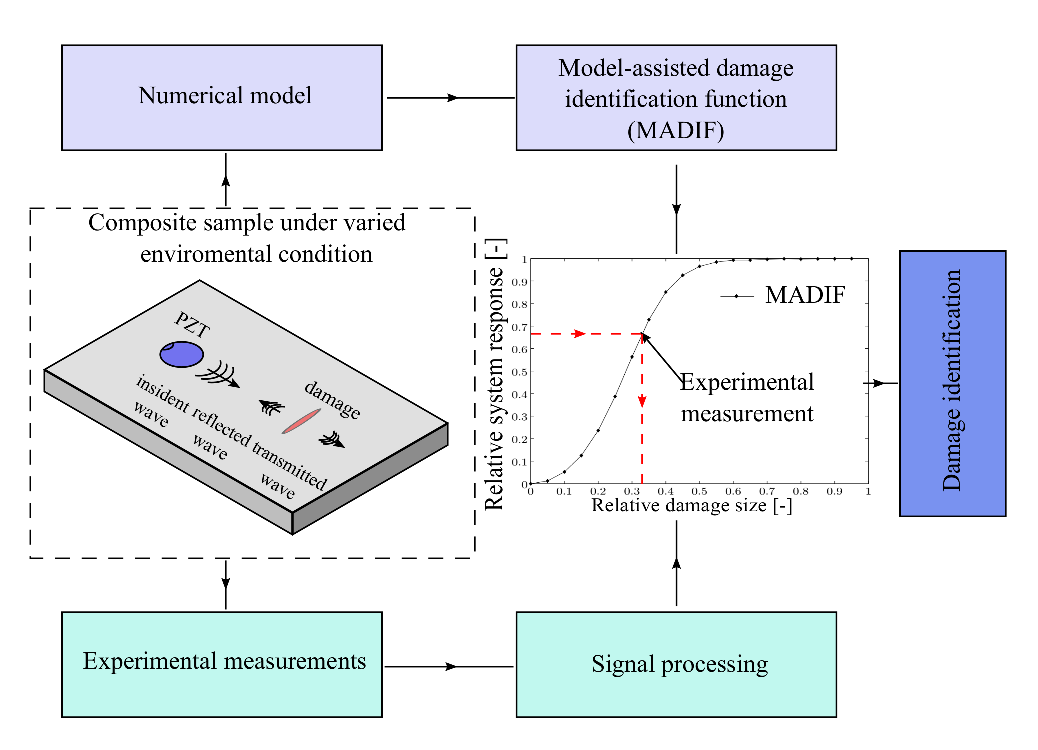
\includegraphics[width=1\textwidth]{../Figures/scheme.eps}
	\caption{Scheme of damage identification based on model--assisted damage identification function (MADIF)}
	\label{fig:scheme}
\end{figure}
The following tasks must be conducted to complete the assumed goals: 
\begin{itemize}
	\item Propose a robust numerical model of the propagating GW in the composite structure under varied ambient temperature and the different boundary conditions,
	\item Experimental validation of the obtained numerical results,
  \item Determination of the model-assisted damage identification function (MADIF) to define damage influence on the propagating waves,
	\item Experimental investigation of the inspected structure,
	\item Propose a framework of the damage detection based on MADIF.
\end{itemize}
\section{Significance of the project}
\subsection{State--of--art}
Currently, researchers have been focused on using a numerical modelling for development and validation of SHM techniques. The numerical simulations were also employed for computation of data sets used in supervised training methods which employ artificial neural networks.

Many existed numerical methods were adopted, or new methods have been developed for the GW propagation analysis during the recent decades. The finite element method (FEM) applied to solve numerous engineering problems has also found application for modelling of wave propagation \cite{talbot1975finite, koshiba1984finite}. The incontestable advantage of this method is a possibility of modelling of structures varied in shape, size, dimension, and boundary conditions. However, due to low order approximation fine meshing is required and an error of the wave propagation increases with the time of the simulation. Other classical methods applied for modelling of elastic waves propagation are the finite difference method (FDM) \cite{strikwerda1989finite} and the boundary element method (BEM) \cite{brebbia2012boundary}. A new method for simulation of GW---local interaction simulation approach (LISA), was presented in \cite{delsanto1992connection}. In this method, a heuristic approach is implemented instead of solving a finite differential equation. On the other hand, Doyle proposed a spectral element method based on fast Fourier transform (FFT SEM) \cite{doyle1989wave}. This technique is very efficient, but it is limited to simple 1D problems.

\begin{figure}
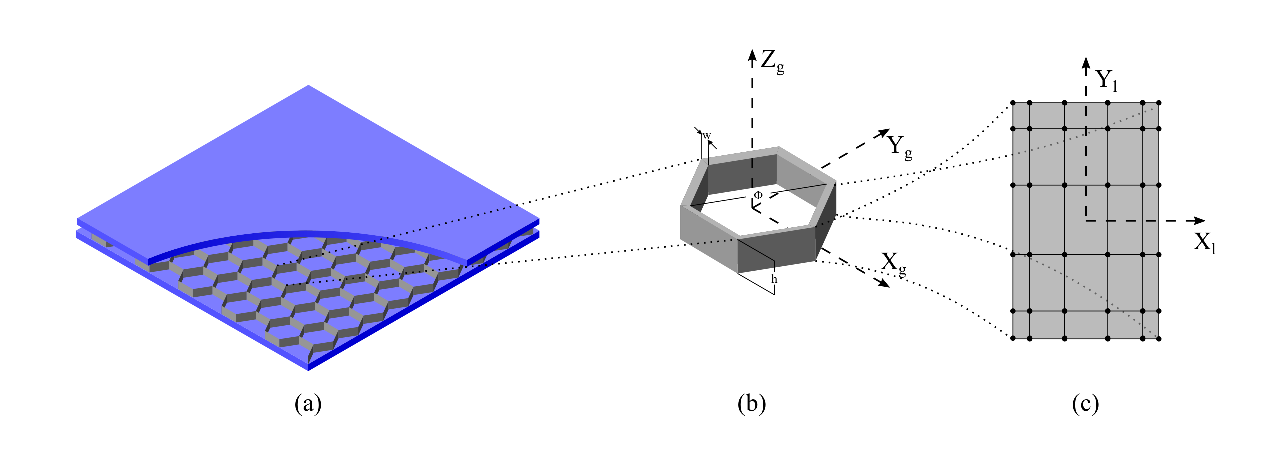
\includegraphics[width=1\textwidth]{../Figures/honeycomb.eps}
	\caption{(a) Composite honeycomb sandwich panel (CHSP), (b) a cell of the honeycomb core, (c) a wall of the cell with distribution of the nodes}
	\label{fig:honeycomb}
\end{figure}
The flexibility of conventional methods was combined with the efficiency of FFT SEM in the formulation of time--domain Spectral Element Method (SEM) proposed by Patera \cite{patera1984spectral}. The SEM was systematically implemented for simulation of elastic waves propagation in various structures, such as rods, beams, plates, etc. \cite{kudela2007modelling, kim2008time, peng2009modeling, ha2009optimizing, schulte2010spectral, rucka2011modelling, ostachowicz2011guided, zak2012damage, ge2014accurate}. Moreover, an electromechanical coupling was realised for modelling a wave excitation/sensing by the piezoelectric transducers.
 
The crucial issue in modelling of GW is an adhesive layer between the transducer and the host structure because it transfers stresses and strains from/to the sensor. According to \cite{crawley1987use}, if the shear modulus increases or thickness decreases shear lag becomes less significant, and shear is effectively transferred mainly near to the end of the PZT. Ha and Chang presented the parametric studies of generating and recording of the GW in an isotropic plate depending on the thickness and material properties of the adhesive layer \cite{ha2010adhesive}. The authors adopted a hybrid spectral element method (i.e. a combination of SEM and Gauss quadrature with two points for formulation mass and stiffness matrices. The numerical method was successfully validated by using experimental measurements conducted in isotropic plates. \cite{ha2009optimizing}. Islam and Huang studied the effects of the adhesive layer on the electromechanical impedance (EMI) of the PZT sensor \cite{islam2014understanding}. The adhesive thickness for optimisation of Lamb waves in SHM was also considered in \cite{willberg2015simulation, islam2016effects}. Taking into consideration the adhesive layer modelled by three--dimensional (3D) elements significantly decreases a required time increment, due to the fact that its thickness is much lower than the dimensions of the remaining components. On the other hand, neglecting the adhesive layer causes that the system response is underestimated. Recently, that issue is under investigation in the work of the project leader.

In the proposed project, it is assumed to take into account composite honeycomb sandwich panel (CHSP) as a host structure. CHSP is a type of structure, which is composed of the mid--core with the geometry of honeycomb bonded between thin composite skins, e.g. carbon fiber reinforced polymer (CFRP), as it is presented in Fig. \ref{fig:honeycomb}(a). In the literature, CHSP is modelled by homogenization of one cell of the honeycomb core (see Fig. \ref{fig:honeycomb}(b)) which is considered as the representative volume element (RVE) \cite{hosseini2013numerical, catapano2014multi, schaal2018core}. In the proposed research, the real geometry of the core will be retained, and each wall of the hexagonal cell will be modelled separately by two--dimensional spectral element (see Fig. \ref{fig:honeycomb}(c)). Such an approach will ensure the authentic character of propagating waves with resonant effect regarding the size of the cell.
\subsection{Innovation}
The novelty of the proposed study can be briefly summarised as follows:
\begin{itemize}
	\item A new approach for damage identification according to the DIF defined by the numerical simulation;\\
		In this proposal, the numerical model is an inherent part of the framework of the damage identification in opposite to many methods available in the literature which rely on experimental signals only. 
	\item A new approach for numerical modelling of the honeycomb composite structure;\\
		The model with the real geometry of the core will be implemented in the scheme of SEM.  
	\item Wave propagation under varied boundary conditions;\\
		There is an evident gap in the literature for the analysis under various boundary conditions because most often researchers assume that all edges are free.. In the proposed model, different boundary conditions will be taken into account.
\end{itemize}
\subsection{Impact}
The proposed project undertakes fundamental safety issues regarding the application of complex composite structures. The results of the investigation will have an impact on the development of worldwide research on SHM. It is expected that a novel technique for damage severity estimation will be developed.
Additionally, the numerical model of the GW propagation in advanced materials such as CHSP under various ambient temperatures and boundary conditions will be improved.

\section{Work plan}
In order to achieve the intended goals, the following research plan will be implemented:
\begin{enumerate}[label=\Roman*.]
	\item Numerical modelling of the baseline.\\
	Selection of the parameters of the simulations:
	\begin{itemize}
		\item dimension and size of elements; 
		\item duration time of propagating waves and time increment used in the explicit solver.
	\end{itemize}
	\item Experimental model validation.
	\begin{itemize}
		\item Experimental measurements at the IMP PAN laboratory.
	\end{itemize}
	\item Determination of the MADIF.
	\begin{itemize}
		\item Selection of the parameter related to damage: type, size, location, orientation;
		\item Selection of inspection method: pitch--catch, pulse--echo;
		\item Selection of the parameter related to the response of the object: the amplitude of the scattered wave, time--of--flight of the wave packet reflected from the defect;
		\item Milestone: MADIF curve.
		\end{itemize}
	\item Experimental investigation of MADIF based damage identification.
	\begin{itemize}
		\item Experimental measurements and signal processing;
		\item Localisation and quantifying the severity of damage based on MADIF;
		\item Analysis and summary of obtained results.
	\end{itemize}
\end{enumerate}
The project schedule is presented on the Gantt chart in Tab \ref{tab:Gantt}.
The crucial issue to successfully implement the plan mentioned above is the accurate and robust model to perform a large number of numerical simulations. The solution would be using 2D elements instead of full 3D implementation or a mix of 2D and 3D elements (i.e. for piezoelectric transducers only). Moreover, computation speed up will be achieved by using parallel calculation on the multi--core graphics processing unit (GPU).
\begin{table}[h]
	\caption{Gantt chart of the research activity}
	\label{tab:Gantt}
	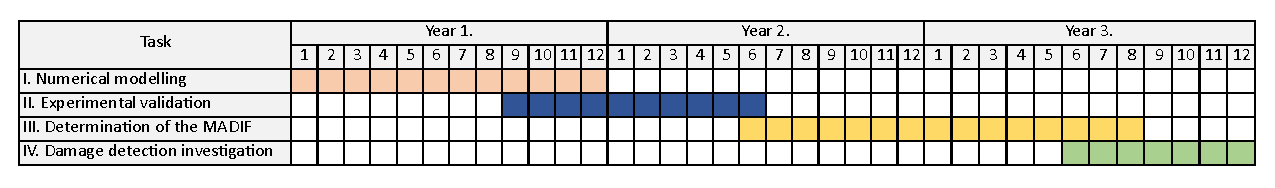
\includegraphics[width=1\textwidth]{../Figures/Gantt.eps}
\end{table}
\section{Methods of research}
\subsection{Spectral Element Method}
The numerical modelling of the GW propagation is a complex and challenging process due to the multimodal and dispersive character of this phenomenon. The appropriate modelling technique should be adaptable to the different type of the structure, accurate in calculation and time efficient. The SEM is one of the methods, which was successfully implemented and fulfils conditions mentioned above. This method, which was developed by Patera \cite{patera1984spectral}, combines the flexibility of finite element method FEM and fast convergence of spectral methods in the frequency domain. The SEM is well known to the leader of the project \cite{fiborek2018time, sikdar2018effects} and the leader's supervisor who is a worldwide expert in the field of modelling the phenomena of elastic wave propagation \cite{kudela2007modelling,kudela20093d,kudela2016parallel} and SHM system \cite{ostachowicz2009damage}.

The idea of SEM is similar to FEM. Both methods use a division of the modelled domain into finite elements, imposing the arbitrary boundary conditions and external forces in the particular nodes. The main difference between those methods is a distribution of nodes in elements and approximation function describing changes of displacements. The element nodes in SEM are non--uniformly distributed and they are coincident with the coordinates of the Gauss--Lobatto--Legendre (GLL) integration points (see Fig. \ref{fig:honeycomb}(c)).
Fig. \ref{fig:shape_function} depicts examples of 2D orthogonal shape functions which are constructed as a tensor product of $N_m(\xi)$ and $N_n(\eta)$:
\begin{figure}
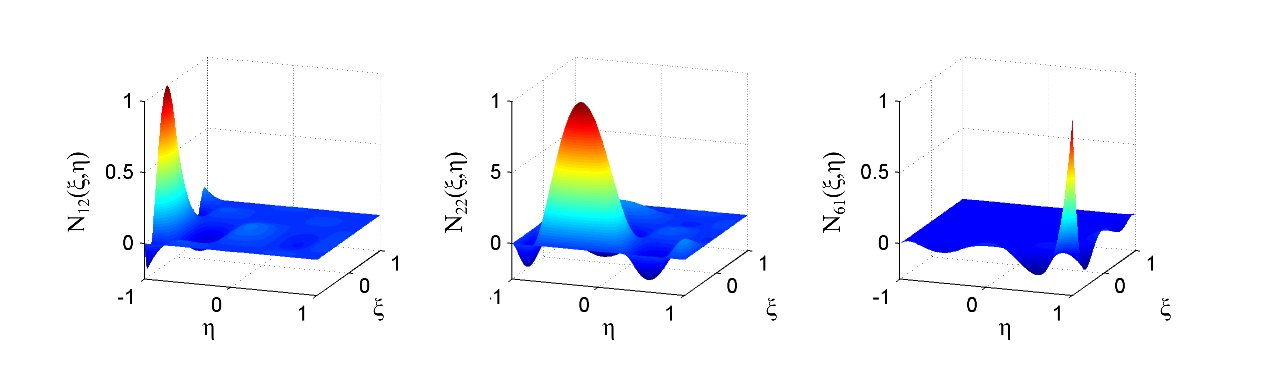
\includegraphics[width=1\textwidth]{../Figures/shape_function.eps}
	\caption{2D shape functions}
	\label{fig:shape_function}
\end{figure}
\begin{equation}
N_{mn}(\xi,\eta)=N_m(\xi)N_n(\eta),\quad for \quad m=1\dots p,n=1\dots r
\label{eq:shape}
\end{equation} 
where $N_m(\xi)$ and $N_n(\eta)$ are the 1D shape functions (the Lagrange polynomials of $p-1$ and $r-1$ order, respectively), and $p$, $r$ denotes the number of nodes along $\xi$ and $\eta$ direction, respectively. As a consequence of orthogonality of shape functions as well as the application of GLL quadrature, the mass matrix is diagonal in the formulation. This property significantly reduces computation time for solving the equation of motion because the central difference scheme is used for the purpose, in which the mass matrix must be inverted.

Numerical modelling of honeycomb sandwich composite usually is realised by the homogenization of material properties. Unfortunately, homogenization causes that the phenomenon of propagation of elastic waves in such structure is often represented with not enough details. While a model based on the 3D theory of elasticity significantly increases the time of computational operations and the need for operational memory, a new approach is proposed. Each wall of the hexagonal cell is modelled separately using 2D spectral elements. The displacements of each wall are calculated in the local system and transferred into the global system through the transformation matrix. Subsequently, the core will join with the skin elements, so that field of displacement of the common geometrical points of both skin and core elements are identical. This type of connection would be implemented through the interface based on Lagrange multipliers. This approach will reduce the number of degrees of freedom, which in turn will shorten the calculation time and reduce the need for operational memory.
\subsection{Simulation under varied boundary and environmental condition}
The composite materials are used in a practical application under a wide range of the ambient temperature. Therefore, in the project, the temperature range between $-40^{\circ} C$ and $+120^{\circ} C$ will be considered. In order to perform a temperature dependent simulations, the elastic moduli of the components will be compensated \cite{sikdar2018study,sikdar2018effects} according to the methodology presented in \cite{chamis1983simplified, salamone2009guided}. While the temperature in the proposed range affects mainly the properties of the polymeric matrix of the CFRP laminate, Chamis proposed the following temperature degradation factor for the stiffness of resin matrices:
\begin{equation}
F_m=\left (\frac{T_{g0}-T}{T_{g0}-T_R}\right)^{1/2}
\label{eq:temp_factor}
\end{equation}
where $T_{g0}$ is the glass transition temperature at the reference temperature $T_R$, and $T$ is the ambient temperature.
Additional the changes of the remaining components, i.e. the piezoelectric transducer and the adhesive layer must be taken into consideration. The temperature characteristics of used materials are available from the manufacturers.
Moreover, during the simulates of GW the global system will be modified by imposing different essential boundary condition.
\subsection{Experimental validation}
The results obtained in the simulations will be verified with the full wavefield measured by the Scanning Doppler Laser Vibrometer (SDLV) in the room temperature. The SDLV is a non--contact technique for the velocity determination of the inspected component by the measurement of the frequency change of light reflected from moving surfaces.

The model with the varied temperature effects will be validated in the climate chamber in the wide range of temperatures (i.e. $-40^{\circ} C$ to $+120^{\circ} C$). Because it is unachievable to take full wavefield by the SDLV in the environmental chamber, the excitation and sensing of the waves will be conducted by the array of piezoelectric transducers permanently attached to the samples.

The following equipment is available in the IMP PAN laboratory:
\begin{itemize}
	\item 3D Scanning Doppler Laser Vibrometer (namely Polytec PSV--400--3D),
	\item Environmental chamber Angelantoni Test Technologies, model MyDiscovery 600 C (internal volume 553l, temperature range [$-75^{\circ} C$; $+180^{\circ} C$] with fluctuation $\pm0.3^{\circ} C$,
	\item Digital oscilloscopes, signal amplifiers, function generators and various types of piezoelectric transducers for elastic wave excitation.
\end{itemize}
\bibliography{../BibTeX_Preludium16}{}
\end{document}